\documentclass[a4paper,12pt,twoside]{memoir}

% Castellano
\usepackage[spanish,es-tabla]{babel}
\selectlanguage{spanish}
\usepackage[utf8]{inputenc}
\usepackage[T1]{fontenc}
\usepackage{lmodern} % scalable font
\usepackage{microtype}
\usepackage{placeins}

\RequirePackage{booktabs}
\RequirePackage[table]{xcolor}
\RequirePackage{xtab}
\RequirePackage{multirow}

% Links
\PassOptionsToPackage{hyphens}{url}\usepackage[colorlinks]{hyperref}
\hypersetup{
	allcolors = {red}
}

% Ecuaciones
\usepackage{amsmath}

% Rutas de fichero / paquete
\newcommand{\ruta}[1]{{\sffamily #1}}

% Párrafos
\nonzeroparskip

% Huérfanas y viudas
\widowpenalty100000
\clubpenalty100000

% Evitar solapes en el header
\nouppercaseheads


\let\tmp\oddsidemargin
\let\oddsidemargin\evensidemargin
\let\evensidemargin\tmp
\reversemarginpar



% Imagenes
\usepackage{graphicx}
\newcommand{\imagen}[2]{
	\begin{figure}[!h]
		\centering
		\includegraphics[width=0.9\textwidth]{#1}
		\caption{#2}\label{fig:#1}
	\end{figure}
	\FloatBarrier
}






\graphicspath{ {./img/} }

% Capítulos
\chapterstyle{bianchi}
\newcommand{\capitulo}[2]{
	\setcounter{chapter}{#1}
	\setcounter{section}{0}
	\setcounter{figure}{0}
	\setcounter{table}{0}
	\chapter*{#2}
	\addcontentsline{toc}{chapter}{#2}
	\markboth{#2}{#2}
}

% Apéndices
\renewcommand{\appendixname}{Apéndice}
\renewcommand*\cftappendixname{\appendixname}

\newcommand{\apendice}[1]{
	%\renewcommand{\thechapter}{A}
	\chapter{#1}
}

\renewcommand*\cftappendixname{\appendixname\ }

% Formato de portada
\makeatletter
\usepackage{xcolor}
\newcommand{\tutor}[1]{\def\@tutor{#1}}
\newcommand{\tutorb}[1]{\def\@tutorb{#1}}
\newcommand{\course}[1]{\def\@course{#1}}
\definecolor{cpardoBox}{HTML}{E6E6FF}
\def\maketitle{
  \null
  \thispagestyle{empty}
  % Cabecera ----------------
\begin{center}
  \noindent
\includegraphics[width=\textwidth]{cabeceraSalud}\vspace{1.5cm}%
\end{center}
  
  % Título proyecto y escudo salud ----------------
  \begin{center}
    \begin{minipage}[c][1.5cm][c]{.20\textwidth}
        
\includegraphics[width=\textwidth]{escudoSalud.pdf}
    \end{minipage}
  \end{center}
  
  \begin{center}
    \colorbox{cpardoBox}{%
        \begin{minipage}{.8\textwidth}
          \vspace{.5cm}\Large
          \begin{center}
          \textbf{TFG del Grado en Ingeniería de la Salud}\vspace{.6cm}\\
          \textbf{\LARGE\@title{}}
          \end{center}
          \vspace{.2cm}
        \end{minipage}
    }%
  \end{center}
  
    % Datos de alumno, curso y tutores ------------------
  \begin{center}%
  {%
    \noindent\LARGE
    Presentado por \@author{}\\ 
    en Universidad de Burgos\\
    \vspace{0.5cm}
    \noindent\Large
    \@date{}\\
    \vspace{0.5cm}
    %Tutor: \@tutor{}\\ % comenta el que no corresponda
    Tutores: \@tutor{} -- \@tutorb{}\\
  }%
  \end{center}%
  \null
  \cleardoublepage
  }
\makeatother



% Datos de portada
\title{Modelado dinámico de la diabetes tipo I y estudio de técnicas de control de la glucosa \\Documentación Técnica}
\author{Marina Sainz Bermejo}
\tutor{Daniel Sarabia Ortiz}
\tutorb{Jesús Enrique Sierra García}
\date{\today}

\begin{document}

\maketitle



\cleardoublepage



%%%%%%%%%%%%%%%%%%%%%%%%%%%%%%%%%%%%%%%%%%%%%%%%%%%%%%%%%%%%%%%%%%%%%%%%%%%%%%%%%%%%%%%%



\frontmatter


\clearpage

% Indices
\tableofcontents

\clearpage

\listoffigures

\clearpage

\listoftables

\clearpage

\mainmatter

\appendix




\apendice{Plan de Proyecto Software}

\section{Introducción}

Se incluye a continuación la planificación seguida a lo largo de este proyecto: a nivel temporal, especificando las tareas realizas, a nivel económico, estimando un coste del trabajo, y de forma breve, a nivel legal, indicando los aspectos necesarios.

\section{Planificación temporal}

Para la planificación temporal de este proyecto, se ha estimado emplear la metodología Scrum, que consiste en un marco de trabajo para la gestión de proyectos, basado en un enfoque iterativo e incremental. El enfoque incremental se refiere a los sprints, ciclos de trabajo de duración fija que van delimitando las tareas del proyecto. Estas tareas han sido recogidas en GitHub en el apartado de issues, y la duración de los sprints comprende de. Por otro lado, el enfoque iterativo permite la mejora y el avance del proyecto, pues la creación continua de nuevos sprints implica haber alcanzado los objetivos del anterior. 

\clearpage
\textbf{Sprint 1} (10/03/2024 – 20/03/2024) 
\begin{enumerate}
    \item[-] \textit{Búsqueda de información}: conocimiento inicial sobre la dinámica glucosa insulina en el organismo, elementos biológicos implicados y mecanismos regulatorios.
    \item[-] \textit{Clasificación de los modelos dinámicos de la glucosa}: búsqueda bibliográfica de los modelos matemáticos que más se ajustan al comportamiento de la glucosa. Encontramos especial relevancia en los Modelos de Bergman y Ackerman, y estudiamos la posibilidad de incluir otras variantes de ellos.
\end{enumerate}

\begin{figure}[htbp]
    \centering
    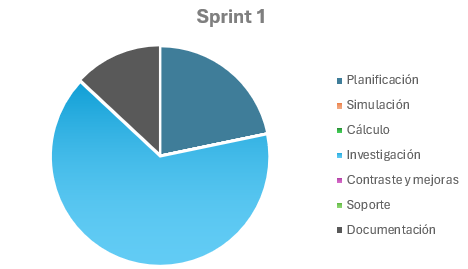
\includegraphics[width=0.8\linewidth]{img/Sprints/1.png}
    \caption{Sprint 1: Distribución de tareas.}
    \label{fig:sprint1}
\end{figure}

\textbf{Sprint 2} (20/03/2024-30/04/2024)
\begin{enumerate}
    \item[-] \textit{Modelado de los modelos matemáticos}: búsqueda exhaustiva de los sistemas de ecuaciones que rigen los modelos seleccionados. Comprensión de las variables y parámetros que los componen.
    \item[-] \textit{Modelo Mínimo de Bergman}: estudio del funcionamiento del modelo. Búsqueda de referencias bibliográficas que permitan comenzar las simulaciones. Reflejo del sistema glucorregulatorio óptimo.
    \item[-]  \textit{Modelo de Ackerman}: estudio del funcionamiento del modelo. Búsqueda de referencias bibliográficas por constituirse como el modelado pionero de la glucosa e insulina.
\end{enumerate}

\begin{figure}[htbp]
    \centering
    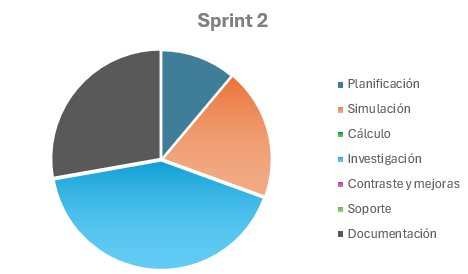
\includegraphics[width=0.8\linewidth]{img/Sprints/2.png}
    \caption{Sprint 2: Distribución de tareas.}
    \label{fig:sprint2}
\end{figure}


\textbf{Sprint 3} (30/03/2024 – 9/04/2024)
\begin{enumerate}
    \item[-] \textit{Formación en Latex}: búsqueda de información sobre el manejo en LaTex. Esta tarea comprende el aprendizaje de la inclusión de gráficas, ecuaciones, tablas, y otros elementos para el trabajo.
    \item[-] \textit{Búsqueda de datos experimentales}: puesta en contacto con el Servicio de Nutrición del Hospital de Burgos (HUBU). Búsqueda de datos de pacientes diabéticos y no diabéticos.
    \item[-]  \textit{Validación de los modelos con datos reales}: issue creado para estudiar el comportamiento de estos modelos con datos reales de pacientes, con la finalidad de observar las diferencias significativas entre ellos.
\end{enumerate}
\clearpage

\begin{figure}[htbp]
    \centering
    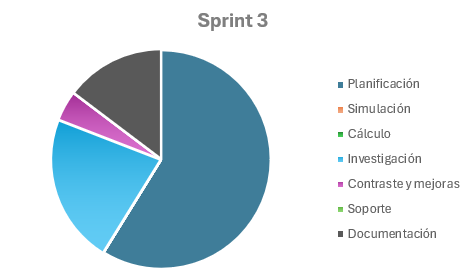
\includegraphics[width=0.8\linewidth]{img/Sprints/3.png}
    \caption{Sprint 3: Distribución de tareas.}
    \label{fig:sprint3}
\end{figure}

\textbf{Sprint 4} (9/04/2024-19/04/2024)
\begin{enumerate}
    \item[-] \textit{Obtención de datos}: anonimización y confidencialidad: Solicitud de datos anonimizados por parte del HUBU. Redacción y envío del Informe Bioético de Protección de Datos. No se ha podido completar esta tarea debido a que no se logró la obtención de los datos. 
    \item[-] \textit{Modelo de Bergman, ejercicio}: inclusión de la variable en el modelo y visualización de resultados iniciales para el comportamiento adecuado del sistema glucorregulatorio.
    \item[-]  \textit{Validación de los modelos con datos reales}: issue creado para estudiar el comportamiento de estos modelos con datos reales de pacientes, con la finalidad de observar las diferencias significativas entre ellos.
\end{enumerate}
\clearpage
\begin{figure}[htbp]
    \centering
    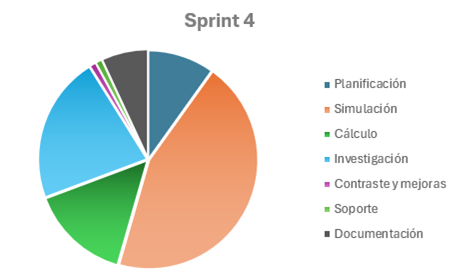
\includegraphics[width=0.8\linewidth]{img/Sprints/4.png}
    \caption{Sprint 4: Distribución de tareas.}
    \label{fig:sprint4}
\end{figure}

\textbf{Sprint 5} (19/04/2024- 29/04/2024)
\begin{enumerate}
    \item[-] \textit{Modelo de Berman Modificado}: revisión bibliográfica de artículos que incluyan otras ecuaciones que permitan modelar de forma más amplia el comportamiento de la glucosa. 
    \item[-] \textit{Insulina exógena}: inclusión de la entrada en el modelo, y estudio de su efecto para pacientes diabéticos.
    \item[-]  \textit{Modelo de Bergman Modificado y perturbaciones}: inclusión de otras variables, como son el ejercicio y la ingesta. Comparación de salidas obtenidas.
\end{enumerate}
\clearpage
\begin{figure}[htbp]
    \centering
    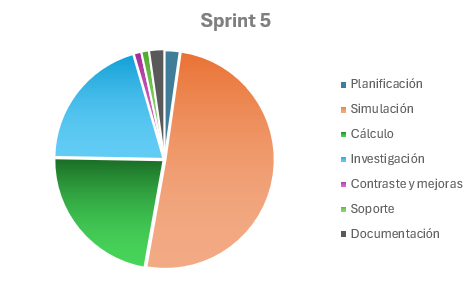
\includegraphics[width=0.8\linewidth]{img/Sprints/5.png}
    \caption{Sprint 5: Distribución de tareas.}
    \label{fig:sprint5}
\end{figure}

\textbf{Sprint 6} (29/04/2024- 9/05/2024)
\begin{enumerate}
    \item[-] \textit{Inclusión de la insulina variable y constante en el modelo}: simulación del Modelo de Bergman para una insulina variable, pues previamente se había considerado únicamente la variable.
    \item[-] \textit{Papel del páncreas en el sistema glucorregulatorio}: se estudia su mecanismo de acción en el organismo.
    \item[-]  \textit{Variación de los parámetros del modelo de Bergman}: se recogen varios análisis, entre los que destaca la tasa de eliminación de glucosa p1.
\end{enumerate}
\clearpage
\begin{figure}[htbp]
    \centering
    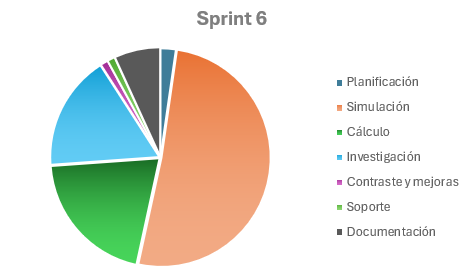
\includegraphics[width=0.8\linewidth]{img/Sprints/6.png}
    \caption{Sprint 6: Distribución de tareas.}
    \label{fig:sprint6}
\end{figure}

\textbf{Sprint 7} (9/05/2024-19/05/2024)
\begin{enumerate}
    \item[-] \textit{Insulina exógena y ejercicio físico}: una vez estudiadas las variables por separado, se combinan ambas para observar su efecto.
    \item[-] \textit{Insulina prolongada y rápida}: se considera el caso de intentar simular las diferentes acciones de la insulina. Se obtiene una estimación.
    \item[-]  \textit{Plan de ingesta completo.}
\end{enumerate}

\begin{figure}[htbp]
    \centering
    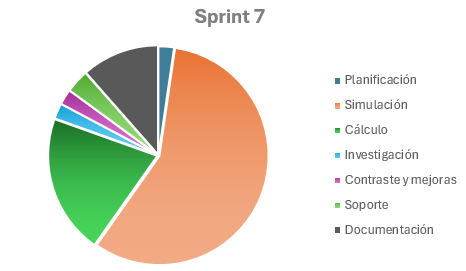
\includegraphics[width=0.8\linewidth]{img/Sprints/7.png}
    \caption{Sprint 7: Distribución de tareas.}
    \label{fig:sprint7}
\end{figure}
\clearpage
\textbf{Sprint 8} (19/05/2024-29/05/2024)
\begin{enumerate}
    \item[-] \textit{Regulador para la insulina, control continuo}: estudio de los mecanismos de control, y de su posible implementación para sustituir la administración manual de la insulina exógena.
\end{enumerate}

\begin{figure}[htbp]
    \centering
    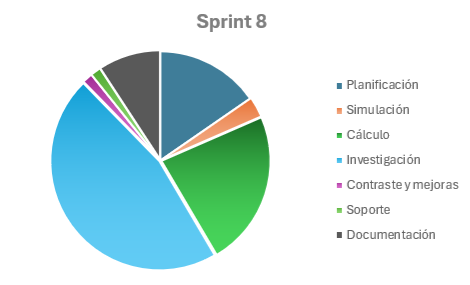
\includegraphics[width=0.8\linewidth]{img/Sprints/8.png}
    \caption{Sprint 8: Distribución de tareas.}
    \label{fig:sprint8}
\end{figure}

\textbf{Sprint 9} (29/05/2024-08/06/2024)
\begin{enumerate}
    \item[-] \textit{Regulador para el modelo de Berman modificado}: se sintonizan un par de reguladores, siguiendo diferentes métodos, para conseguir un control glucémico.
    \item[-] \textit{Latex, memoria y anexo}: se redacta de forma final los documentos, a partir de otros menores que se han ido redactando a lo largo del proyecto.
    \item[-]  \textit{Discusión de los resultados} una vez obtenidas todas las simulaciones llevadas a cabo en el estudio.
\end{enumerate}
\clearpage
\begin{figure}[htbp]
    \centering
    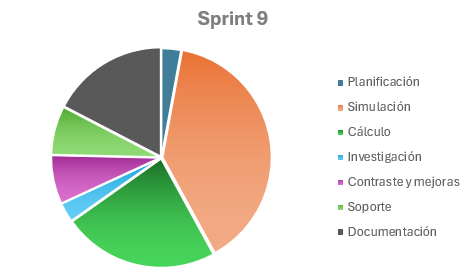
\includegraphics[width=0.8\linewidth]{img/Sprints/9.png}
    \caption{Sprint 9: Distribución de tareas.}
    \label{fig:sprint9}
\end{figure}

\textbf{Sprint 10} (08/06/2024-28/06/2024: Doble Sprint)
\begin{enumerate}
    \item[-]  \textit{Discusión de los resultados.} Ampliación de este issue con el fin de completar y orientar de manera más precisa el estudio. 
\end{enumerate}
\begin{figure}[htbp]
    \centering
    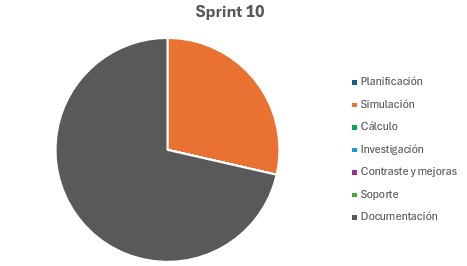
\includegraphics[width=0.8\linewidth]{img/Sprints/10.PNG}
    \caption{Sprint 10: Distribución de tareas.}
    \label{fig:sprint10}
\end{figure}
\clearpage
\section{Planificación económica}


Se indicarán para este apartado los costes tanto personales, como de materiales y desarrollo del proyecto.

Se comienza analizando el sueldo de un ingeniero promedio al salir de la carrera, obtenido en \cite{talent_com}\footnote{La conversión llevada a cabo se ha realizado con el calculador \cite{taxscouts}}:

\begin{table}[htbp]
    \centering
    \caption{Sueldo de un ingeniero en España y sus retenciones}
    \begin{tabular}{|c c|}
        \hline
        Sueldo bruto anual & 30000 \texteuro   \\
        Retenciones por IRPF & 4920 \texteuro \\
        Contribuciones a la Seguridad Social & 1935 \texteuro\\
        Tipo de retención & 16.40\% \\
        Sueldo neto anual & 23.145 \texteuro \\
        \hline
    \end{tabular}
    \label{tab:salario_ingeniero}
\end{table}

Tal y como se especifica para la elaboración del TFG, se estima el empleo de 360 horas en su realización, calculando el precio por hora. Se detallan en la Tabla \ref{tab:coste_personal} los costes personales para el proyecto \footnote{Datos obtenidos de la tabla anterior \ref{tab:salario_ingeniero}}.

\begin{table}[htbp]
    \centering
    \caption{Resumen de los costes personales para el proyecto.}
    \begin{tabular}{|c c|}
        \hline
        Sueldo al mes  & 1928,75 \texteuro   \\
        Sueldo por hora & 12,05 \texteuro \\
        Total por horas realizadas (360) & 4339,68 \texteuro\\
        \hline
    \end{tabular}
    \label{tab:coste_personal}
\end{table}

Se incluyen a continuación el resto de costes del proyecto a nivel material \footnote{Para más información de licencias de Office, entrar en \cite{microsoft}}. Se compone del coste del hardware (ordenador) y el software, que incluye la lincencia de Windows 10 Pro, el Paquete de Office, para redacción inicial de secciones así como elaboración de gráficos circulares, y la aplicación de Matlab, que contiene Simulink \footnote{Precios de Matlab: \cite{mathworks}.}.
\clearpage
\begin{table}[htbp]
    \centering
    \caption{Resumen de los costes materiales para el proyecto.}
    \begin{tabular}{|c c|}
        \hline
        Ordenador HP  & 698 \texteuro   \\
        Licencia Windows 10 Pro & 0 \texteuro (incluida) \\
        Paquete Office & 16,80 \texteuro\\
        Matlab y Simulink & 300 \texteuro\\
       Total material & 1014,8 \texteuro\\
        \hline
    \end{tabular}
    \label{tab:costes_mat}
\end{table}

Obteniendo un coste final:

\begin{table}[htbp]
    \centering
    \caption{Coste final del proyecto}
    \begin{tabular}{|c c|}
        \hline
       Costes personales  & 4339,68 \texteuro   \\
       Costes materiales & 1014,8 \texteuro \\
       \textbf{Total costes proyecto} & \textbf{5354,48} \texteuro\\
       \hline
    \end{tabular}
    \label{tab:costes_totales}
\end{table}

\section{Viabilidad legal}

Respecto a este apartado, siendo un estudio y al no haber empleado datos personales y reales de pacientes, simplemente hay que destacar: 
\begin{enumerate}
    \item[-] Programas de software abierto, como GitHub y Overleaf, no requieren de ninguna licencia específica. Para ambas se trabaja con la versión online, no siendo necesario llevar a cabo ninguna descarga ni asumir ningún coste para su uso.
    \item[-] Las licencias correspondientes al paquete Office requieren de contratación, que en este caso no ha sido necesaria por ser miembro de la Universidad de Burgos (UBU). Se diferencia por tanto la licencia académica y la comercial.
    \item [-] Respecto al programa más empleado para este estudio, MatLab, y su herramienta Simulink, requieren de una licencia para su uso, que en este caso no ha sido necesaria por el mismo motivo que en el apartado anterior. MATLAB y Simulink son productos de MathWorks y están sujetos a términos de uso específicos que se deben cumplir. Concretamente:
    \begin{enumerate}
        \item[-] Las licencias académicas de MATLAB, como es este caso, están diseñadas para ser utilizadas en actividades académicas, tales como la enseñanza, la investigación y el aprendizaje. Usos distintos a los mencionados no estan permitidos para esta modalidad. 
        \item [-] Estas licencias están limitadas a profesores, alumnos y figuras de la institución educativa determinadas. No está permitido el uso a personas ajenas a ellos.
        \item [-] No está permitido utilizar MatLab con licencia académica para desarrollar productos comerciales o realizar actividades lucrativas.
        \item[-] Está prohibida la distribución de sofware ni el uso a personas ajenas a la institución. 
    \end{enumerate}
\end{enumerate}

\apendice{Documentación de usuario}

\section{Requisitos software y hardware para ejecutar el proyecto.}

El principal requisito de software para poder realizar este proyecto es la instalación de MatLab en el ordenador. Simulink, como se ha comentado, es una plataforma de software integrada en MATLAB que se utiliza para modelar, simular y analizar sistemas dinámicos

Para mi caso, se ha trabajado con la versión MatLab R2019 Update 9 (9.7.0.1737446) para Windows de 64-bit (win64), lanzada el 5 de agosto de 2021. Esta versión requiere de los siguientes requisitos:
\begin{enumerate}
    \item \textbf{Requisitos operativos}: en cuanto a sistemas operativos, es compatible en Windows (Windows 10,7, Server 2016 y Server 2019), Mac (10.12,10.13,10.14) y Linux (Ubuntu 18.04, 16.04 LTS, Delbian 9). Es compatible además con los navegadores Microsoft Edge, Firefox, Google Chrome y Safari.
    \item \textbf{Requisitos de hardware}: procesador de 64 bits, memoria mínimo de 4 GB de RAM (8 recomendados), y espacio en disco mínimo para la instalación de 3.2 GB.
    \item \textbf{Control System Toolbox }para el análisis, diseño y sintonización de los sistemas de control. Sus especificaciones son similares a las de MatLab.
\end{enumerate}


\section{Instalación / Puesta en marcha}

La guía de instalación de MatLab viene incluida en la referencia \cite{mathworks2019}.

\section{Manuales y/o Demostraciones prácticas}

Se adjunta a continuación un \textit{breve} manual de uso básico de MatLab, y especialmente, Simulink.

Al abrir MatLab nos encontramos con la siguiente página de inicio:

\begin{figure}[htbp]
    \centering
    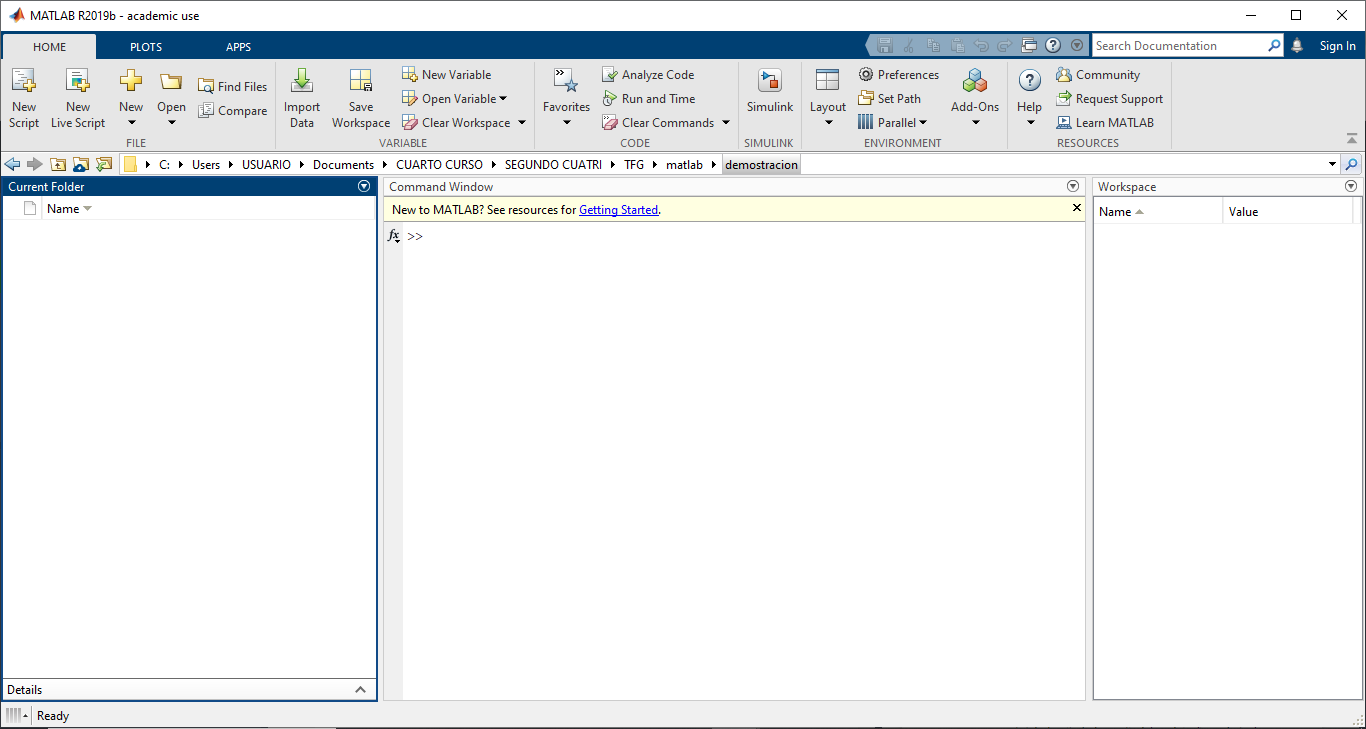
\includegraphics[width=1.1\linewidth]{img/anexos/manual/inicio.PNG}
    \caption{Página de inicio de MatLab.}
    \label{fig:inicio_matlab}
\end{figure}

Para crear o abrir scrips, en el \textbf{\textit{Panel HOME}} se pulsa \textit{New Script} (para crear nuevos) o bien \textit{Open} (para abrirlos desde una carpeta):
\clearpage

\begin{figure}[htbp]
    \centering
    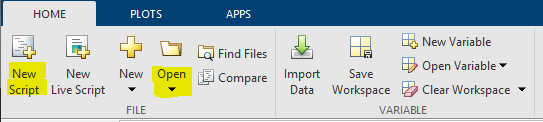
\includegraphics[width=0.8\linewidth]{img/anexos/manual/archivo.PNG}
    \caption{Crear un script en MatLab.}
    \label{fig:crear_script}
\end{figure}

Una vez abierto el script, como se muestra en, se prueba que al ejecutarlo mediante Run aparece la ejecución de dicho archivo en MatLab.

\begin{figure}[htbp]
    \centering
    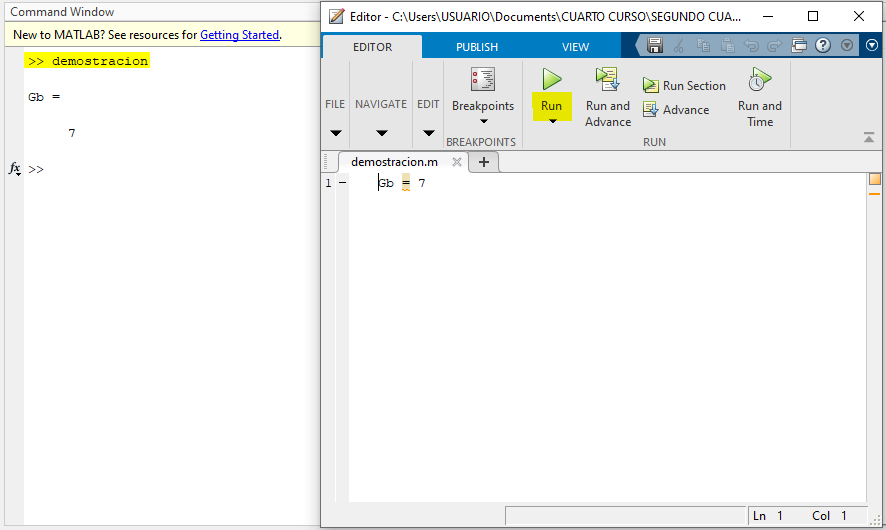
\includegraphics[width=0.8\linewidth]{img/anexos/manual/ej.PNG}
    \caption{Ejecución de un script en MatLab.}
    \label{fig:ejecutar_script}
\end{figure}

Para abrir Simulink, en el \textbf{\textit{Panel HOME}} se pulsa \textit{Simulink} (Figura \ref{fig:abrir_simulink}) y, una vez en la \textit{Simulink Start Page} se abre un \textit{"Blank Model"} (Figura \ref{fig:simulink}).

\begin{figure}[htbp]
    \centering
    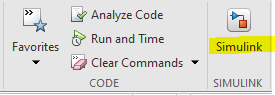
\includegraphics[width=0.5\linewidth]{img/anexos/manual/simulink.PNG}
    \caption{Abrir Simulink en MatLab.}
    \label{fig:abrir_simulink}
\end{figure}
\clearpage
\begin{figure}
    \centering
    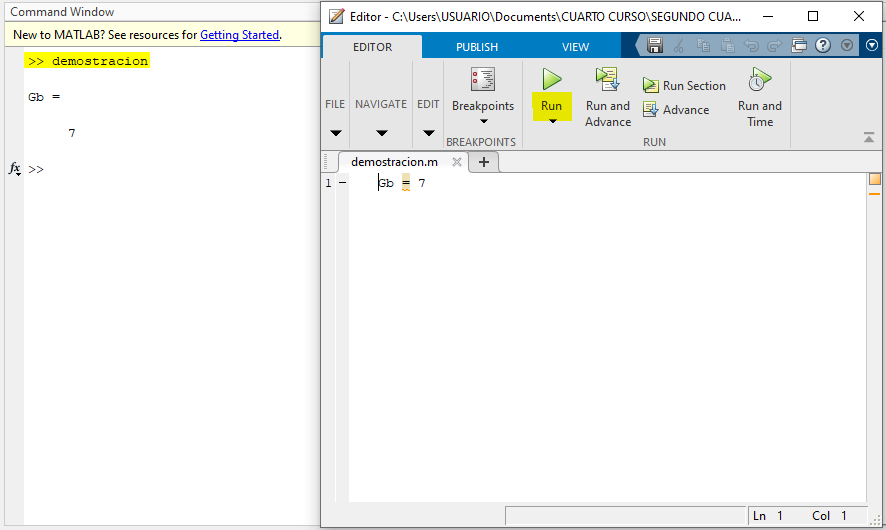
\includegraphics[width=1.1\linewidth]{img/anexos/manual/ej.PNG}
    \caption{Simulink Start Page.}
    \label{fig:simulink}
\end{figure}

Dentro de Simulink (Figura \ref{fig:inicio_simulink}) , se encuentra el marco de trabajo donde se ha realizado este estudio. La librería Simulink Library Browser de la Figura \ref{fig:library_simulink}, es una ventana dentro del entorno de Simulink que proporciona acceso a una amplia variedad de bloques predefinidos y funciones para construir modelos de simulación. 
\clearpage
\begin{figure}[htbp]
    \centering
    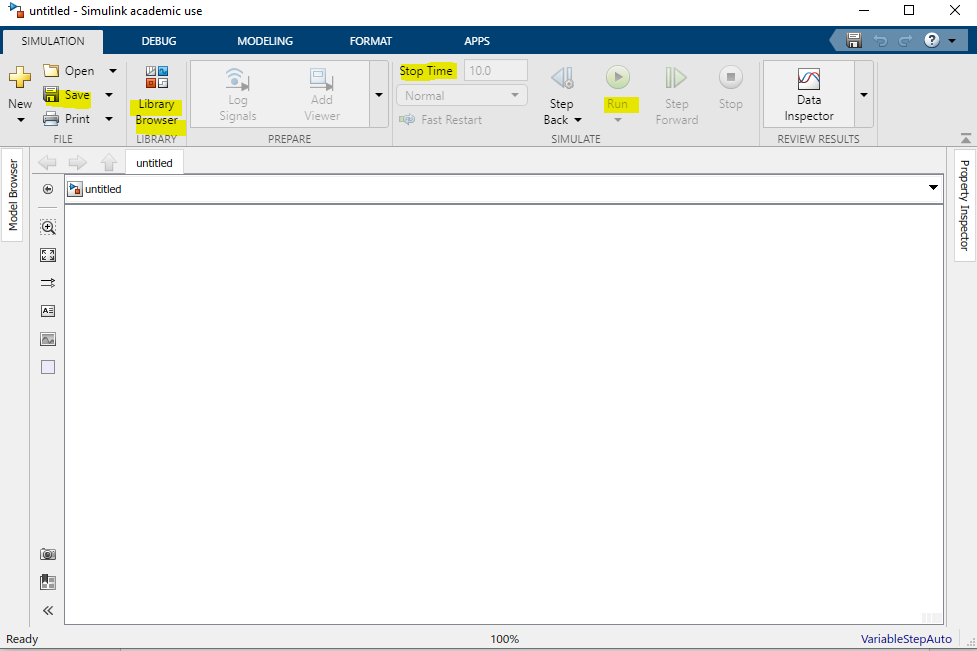
\includegraphics[width=1.1\linewidth]{img/anexos/manual/simulink_start.PNG}
    \caption{Página de inicio de Simulink.}
    \label{fig:inicio_simulink}
\end{figure}
\clearpage
\begin{figure}[htbp]
    \centering
    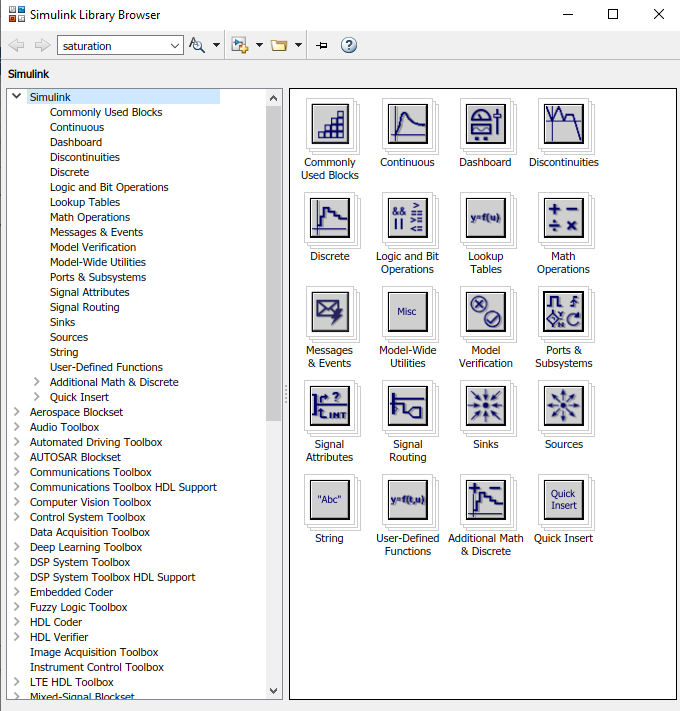
\includegraphics[width=0.9\linewidth]{img/anexos/manual/library.PNG}
    \caption{Simulink Library Browser.}
    \label{fig:library_simulink}
\end{figure}

Mediante \textit{"Stop Time"} se define la duración de la simulación a realizar en segundos, y mediante \textit{"Run"} se ejecuta la simulación. La inclusión de los bloques se realiza arrastrándoles hacia el marco de trabajo.

Se incluyen a continuación los bloques más relevantes para este proyecto:
\begin{enumerate}
    \item Bloques \textit{Sum, Substract, Product, Divide} para realizar operaciones matemáticas básicas.
     \item Bloque \textit{Integrador/Integrator}, para modelar las ecuaciones diferenciales de los modelos matemáticos.
     \item Bloques\textit{ Constant} y \textit{Gain}, para incluir parámetros constantes.
     \item Bloques \textit{Rampa/Ramp, Escalón/Step} para generar señales de entrada.
     \item Bloque\textit{ Scope}, para crea gráficas con las salidas resultantes.
\end{enumerate}

Para guardar los archivos basta con presionar \textit{CONTROL + S}.

Para más información consultar los tutoriales de MatLab en \cite{matlab_intro}.
\apendice{Manual del investigador} % usar el término que mejor se corresponda.
Se propone un despligue de sección alternativo debido a la naturaleza del proyecto.

\section{Diagramas de bloques}

Se incluyen las principales implementaciones llevadas a cabo en Simulink.
\clearpage
\subsection{Modelo de Bergman}

Para el Modelo de Bergman, se han implementado las ecuaciones diferenciales del modelo (\ref{eq:ecBergGluc}) y (\ref{eq:ecBergInsAc}) en Simulink. Se presentan las 2 ecuaciones unidas a sus respectivas gráficas, así como las entradas conectadas a los niveles basales de glucosa e insulina.

\begin{figure}[htbp]
    \centering
    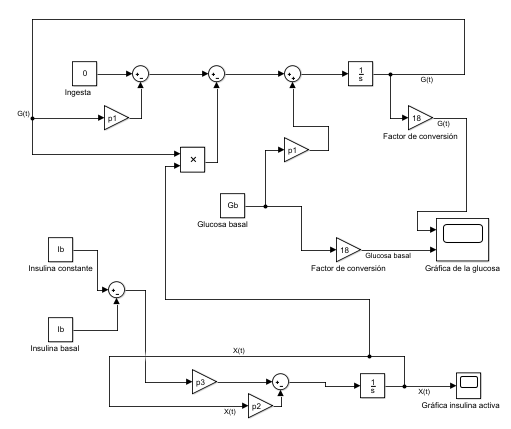
\includegraphics[width=0.9\linewidth]{img/anexos/bloques/modelo_bergman.png}
    \caption{Diagrama de bloques para el Modelo de Bergman.}
    \label{fig:diag_bergman}
\end{figure}

La equivalencia de la Figura \ref{fig:diag_bergman} a nivel matemático es:
\begin{align}
    \frac{dG(t)}{dt}= -p_1 (G(t) - G_b) - X(t)G(t) , G(0) = Gb
    \label{eq:ecBergGluc}\\
    \frac{dX(t)}{dt}= -p_2 X(t) + p_3(I(t) - I_b),    X(0) = 0
    \label{eq:ecBergInsAc}
\end{align}
\clearpage
Cuando no se trabaja con una insulina constante, se añade una tercera ecuación al sistema, que modela la insulina a lo largo del tiempo. También tiene caracter diferencial y permite aproximar a la realidad el comportamiento de la glucosa e insulina en el organismo. 
Se añade al sistema anterior formado por las ecuaciones (\ref{eq:ecBergGluc}) y (\ref{eq:ecBergInsAc}), la ecuación (\ref{eq:insulina_variable}), representada en la Figura \ref{fig:diag_ins_var}.

\begin{equation}
    \frac{dI(t)}{dt} = p_6 (G(t)-p_5)^+ t -n(I(t)+Ib), Ib(0)=0
    \label{eq:insulina_variable}
\end{equation}

\begin{figure}[htbp]
    \centering
    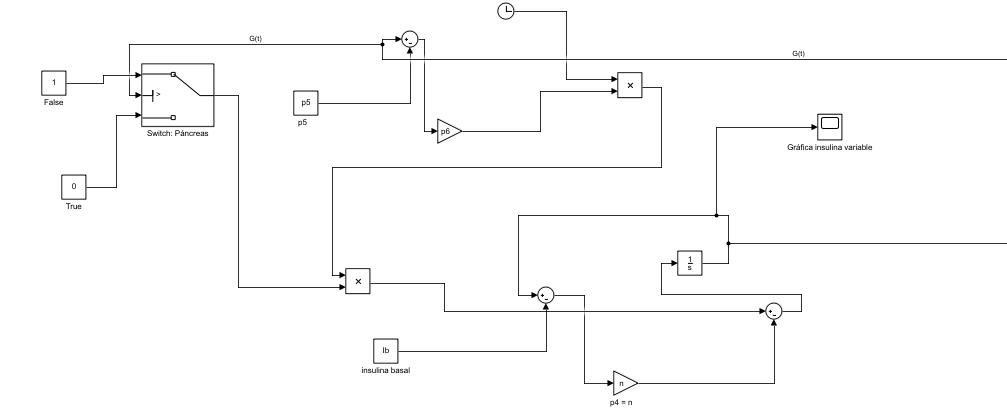
\includegraphics[width=1\linewidth]{img/anexos/bloques/ins_variable.png}
    \caption{Diagrama de bloques de la insulina variable en el Modelo de Bergman.}
    \label{fig:diag_ins_var}
\end{figure}

Se muestra en la Figura el Modelo de Bergman completo con la insulina I(t) variable modelada en la Figura \ref{fig:diag_ins_var}.
\clearpage

\begin{figure}[htbp]
    \centering
    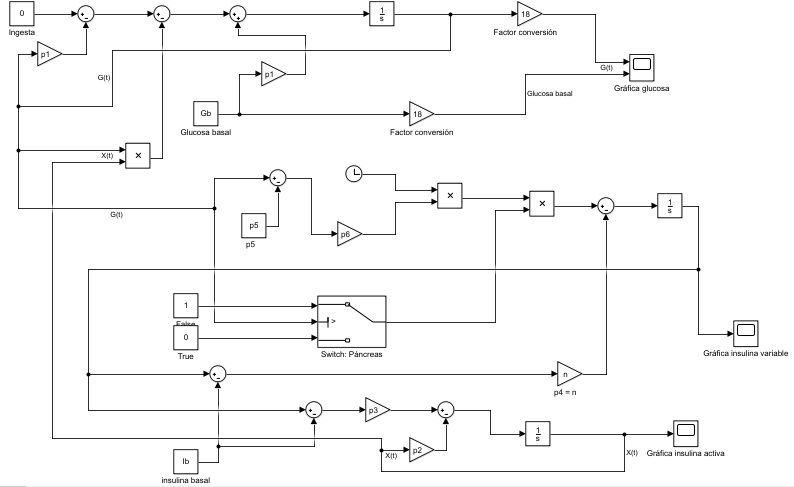
\includegraphics[width=1.2\linewidth]{img/anexos/bloques/insulina_var_completo.PNG}
    \caption{Diagrama de bloques del Modelo de Bergman con insulina variable.}
    \label{fig:diag_ins_var_completo}
\end{figure}
\clearpage
\subsection{Modelo Modificado}

Para el Modelo de Bergman Modificado, se lleva a cabo una variación en la ecuación de la insulina (\ref{eq:ecBergMod}) con el fin de incluir la variable insulina exógena U. 

De esta forma, el sistema resultante del Modelo Modificado es el siguiente:

\begin{align}
    \frac{dG(t)}{dt}= -p_1 (G(t) - G_b) - X(t)G(t), G(0)=Gb \\ \label{eq:glucosa_mod_mod}
    \frac{dX(t)}{dt}= -p_2 X(t) + p_3(I(t) - I_b), X(0) = 0 \\
    \frac{dI(t)}{dt}= -n I(t) + \frac{U(t)}{Vi}, I(0) = Ib 
    \label{eq:ecBergMod}
\end{align}

Se muestra en la Figura \ref{fig:diag_mod_bergman} el diagrama de bloques empleado.

\begin{figure}[htbp]
    \centering
    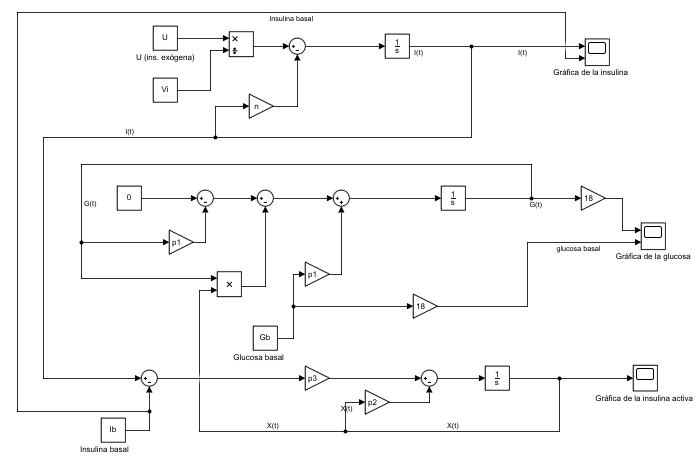
\includegraphics[width=1\linewidth]{img/anexos/completo_bergman_modificado.png}
    \caption{Diagrama de bloques para el Modelo Modificado de Bergman.}
    \label{fig:diag_mod_bergman}
\end{figure}
\clearpage
Se incluye a continuación la implementación de las funciones ingesta (Figura \ref{fig:diag_ingesta}) y ejercicio físico (Figura \ref{fig:diag_ejercicio}) para el Modelo Modificado de Bergman. Ambas se encuentran unidas a la entrada del sistema, que es el tiempo, representado mediante un bloque \textit{Clock}. Además, se introducen como bloques denominados \textit{MatLab Function}.

\begin{figure}[htbp]
    \centering
    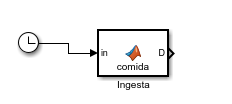
\includegraphics[width=0.5\linewidth]{img/anexos/bloques/ingesta.png}
    \caption{Inclusión de la ingesta en el Modelo Modificado.}
    \label{fig:diag_ingesta}
\end{figure}

\begin{figure}[htbp]
    \centering
    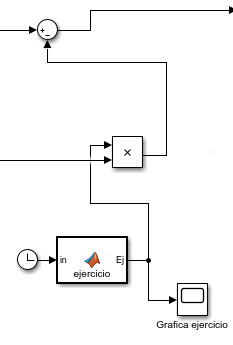
\includegraphics[width=0.4\linewidth]{img/anexos/bloques/ejercicio.png}
    \caption{Inclusión del ejercicio en el Modelo Modificado.}
    \label{fig:diag_ejercicio}
\end{figure}
Ambas variables y sus bloques incluidos en el Modelo Modificado se encuentran en la Figura \ref{fig:diag_completo_modificado}, así como el sistema de ecuaciones \ref{eq:ejercicio_ing_comp} formado.
\clearpage

\begin{align} 
    \frac{dG(t)}{dt}= -p_1 (G(t) - G_b) - X(t)Ej(t)G(t)+D(t), G(0)=Gb \\
    \frac{dX(t)}{dt}= -p_2 X(t) + p_3(I(t) - I_b), X(0) = 0 \\
    \frac{dI(t)}{dt}= -n I(t) + \frac{U(t)}{Vi}, I(0) = Ib \\
    \label{eq:ejercicio_ing_comp}
\end{align}

\begin{figure}[htbp]
    \centering
    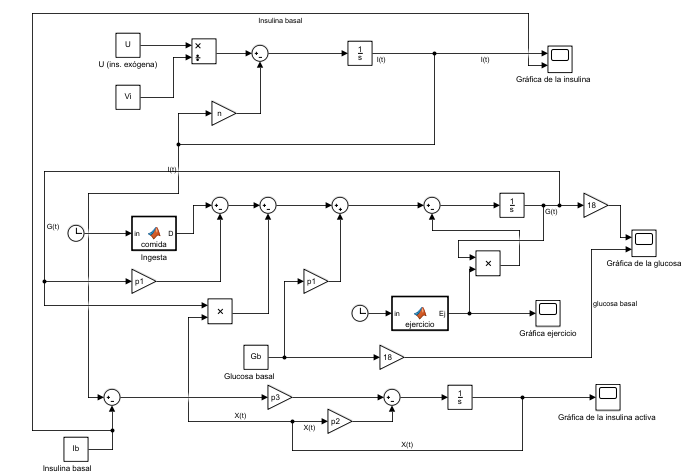
\includegraphics[width=1\linewidth]{img/anexos/bloques/mod_bergman_ej_ing.PNG}
    \caption{Diagrama de bloques del Modelo Modificado con el ejercicio físico y la ingesta.}
    \label{fig:diag_completo_modificado}
\end{figure}

\clearpage
El intento de modelización de la insulina rápida en el Modelo Modificado de Bergman se basa en el uso de un bloque \textit{Switch} conectado a una entrada (la glucosa G(t)), cuya salida puede ser True o False. Además, registra en su interior un umbral de glucosa, simulando el comportamiento del páncreas para el sistema.

\begin{figure}[htbp]
    \centering
    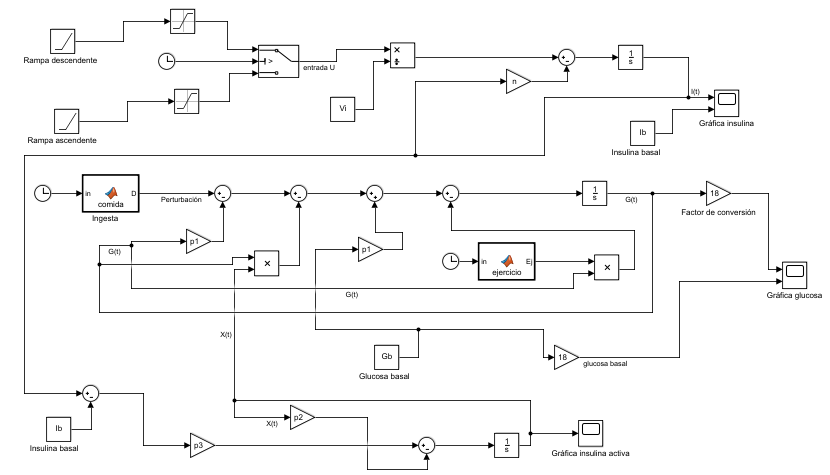
\includegraphics[width=1\linewidth]{img/anexos/bloques/completo_bergman_mod.PNG}
    \caption{Inclusión de la insulina rápida en el modelo.}
    \label{fig:diag_ins_rapida}
\end{figure}
\clearpage
\subsection{Regulación}

Respecto a este apartado, para introducir elementos regulatorios en Simulink basta con emplear el bloque \textit{PID Controller} y establecer los parámetros para los términos proporcional, integral y derivativo en su interior. Su salida se une a la entrada de la ecuación de la insulina, sustituyendo esta nueva unión por la insulina exógena que se administraba anteriormente.

Este implementación se puede observar en la Figura \ref{fig:diag_reg}.

\begin{figure}[htbp]
    \centering
    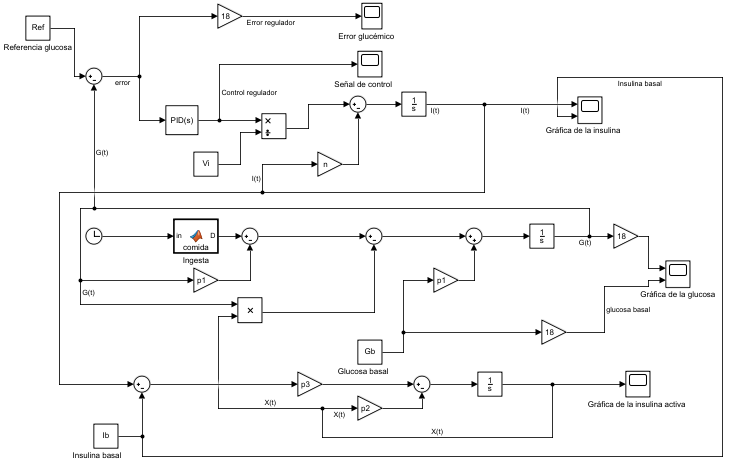
\includegraphics[width=1\linewidth]{img/anexos/bloques/regulacion_bueno.PNG}
    \caption{Inclusión de un regulador en el Modelo Modificado.}
    \label{fig:diag_reg}
\end{figure}

En función de las particularidades de cada regulador, se completan sus términos proporcional, integral y derivativo haciendo \textit{click} dentro del \textit{PID Controller}.

\clearpage

\section{Scripts}

Se incluyen a continuación los scrips ejecutados para llevar a cabo este análisis. Inicialmente, se encuentran los que inicializan las variables de un paciente no diabético (Figura \ref{fig:script_no_diab}), así como de un paciente diabético (Figura \ref{fig:script_diab}).

\begin{figure}[htbp]
    \centering
    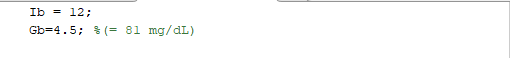
\includegraphics[width=0.8\linewidth]{img/anexos/codigo/no_Diabetico.PNG}
    \caption{Código para el establecimiento de los valores de un paciente no diabético.}
    \label{fig:script_no_diab}
\end{figure}
\begin{figure}[htbp]
    \centering
    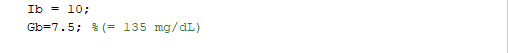
\includegraphics[width=0.8\linewidth]{img/anexos/codigo/diabetico.PNG}
    \caption{Código para el establecimiento de los valores de un paciente diabético.}
    \label{fig:script_diab}
\end{figure}


\subsection{Modelo de Bergman}

\subsubsection{Parámetros del Modelo}

El script necesario para inicializar los parámetros del Modelo se encuentra en la siguiente Figura \ref{fig:script_parametros}:

\begin{figure}[htbp]
    \centering
    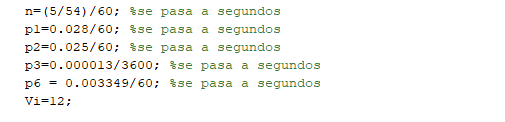
\includegraphics[width=0.8\linewidth]{img/anexos/codigo/p1_p2.PNG}
    \caption{Código para inicializar los parámetros del Modelo de Bergman.}
    \label{fig:script_parametros}
\end{figure}
\clearpage
El estudio de la variación de los parámetros p1, p2 y p3 se recoge en la siguiente Figura \ref{fig:script_var_param}:

\begin{figure}[htbp]
    \centering
    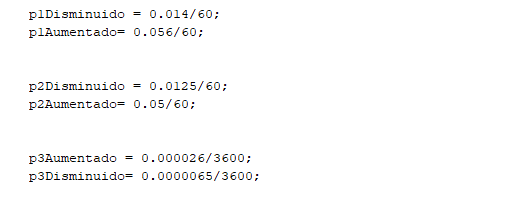
\includegraphics[width=0.8\linewidth]{img/anexos/codigo/variacion_param.PNG}
    \caption{Código para estudiar la variabilidad de los parámetros p1, p2 y p3 del Modelo de Bergman.}
    \label{fig:script_var_param}
\end{figure}


\subsection{Modelo Modificado}

A continuación, se detallan los scripts base correspondientes a las funciones ingesta y ejercicio físico (Figura \ref{fig:script_ingesta} y Figura \ref{fig:script_ejercicio}, respectivamente) , que se han visto modificados a lo largo de las secciones para realizar las distintas simulaciones. 

\begin{figure}[htbp]
    \centering
    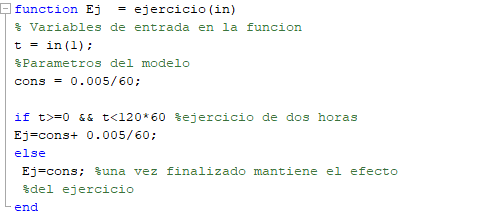
\includegraphics[width=0.8\linewidth]{img/anexos/codigo/funcion_ejercicio.png}
    \caption{Código de la función ejercicio para el Modelo Modificado.}
    \label{fig:script_ejercicio}
\end{figure}
\clearpage
\begin{figure}[htbp]
    \centering
    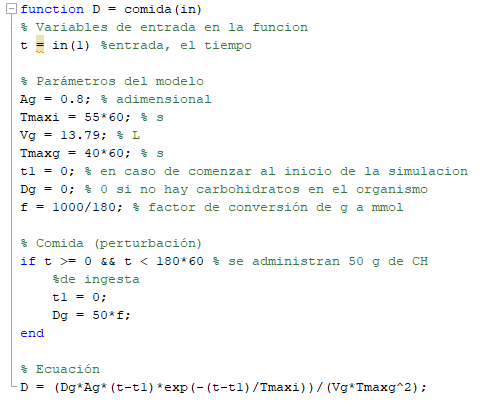
\includegraphics[width=0.8\linewidth]{img/anexos/codigo/funcion_ingesta.png}
    \caption{Código de la función ingesta para el Modelo Modificado.}
    \label{fig:script_ingesta}
\end{figure}

Por último para este apartado, para estudiar la variación de la constante de tiempo n se emplea el script de la Figura \ref{fig:script_n}:

\begin{figure}[htbp]
    \centering
    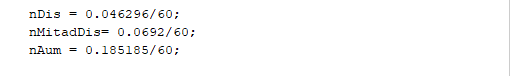
\includegraphics[width=0.8\linewidth]{img/anexos/codigo/variacion_n.PNG}
    \caption{Código para estudiar la variabilidad del parámetro n del Modelo de Bergman.}
    \label{fig:script_n}
\end{figure}



\apendice{Descripción de adquisición y tratamiento de datos}


\section{Tablas y asociaciones}

Se incluyen a continuación las tablas y asociaciones de los datos llevadas a cabo en este proyecto. 

\subsection{Modelo de Bergman}

Para el Modelo de Bergman, los valores empleados para el estudio de la varaición del umbral de liberación de insulina por el páncreas (parámetro $p_5$) se encuentran en la Tabla \ref{tab:p5}, mientras que aquellos empleados para el estudio de la variación de la tasa de eliminación de la glucosa $p_1$, así como $p_2$ y $p_3$, se incluyen en la Tabla \ref{tab:p123}.

\begin{table}[htbp]
    \centering
    \caption{Valores de $p_5$ comparados.}
    \begin{tabular}{|c|c|c|}
        \hline
          & mg/dL & mmol/L  \\
        \hline
        Caso 1 & 81 & 4.5  \\
        Caso 2 & 85 & 4.722  \\
        Caso 3 & 90 & 5 \\
        Caso 4 & 95 & 5.278 \\
        Caso 5 & 100 & 5.56 \\
        \hline
    \end{tabular}
    \label{tab:p5}
\end{table}

\begin{table}[htbp]
    \centering
    \caption{Valores de p1,p2,p3 empleados en las simulaciones.}
    \begin{tabular}{|c|c|c|c|c|}
        \hline
          & Valor base & Valor aumentado & Valor disminuido \\
        \hline
        p1 & 0.028 & 0.056 & 0.014 \\
        p2 & 0.025 & 0.05 & 0.0125 \\
        p3 & 0.000013 & 0.000026 & 0.0000065 \\
        \hline
    \end{tabular}
    \label{tab:p123}
\end{table}

La simulación correspondiente a la variación de los parámetros p2 y p3 se encuentra en la Sección \ref{sec:variacion_p23} de este anexo.

\subsection{Modelo Modificado}

Respecto a la variación de la constante de tiempo n, los valores empleados para la simulación se disponen en la Tabla \ref{tab:pn}:

\begin{table}[htbp]
    \centering
    \caption{Valores n empleados en la simulación.}
    \begin{tabular}{|c|c|}
        \hline
        Caso & Valor \\
        \hline
        n base & $\frac{5}{54} $\\
        n aumentado (nAum) & $2 \times \frac{5}{54} $\\
        n mitad disminuido (nMitadDis) & $\frac{3}{4} \times \frac{5}{54}$ \\
        n disminuido(nDis) & $\frac{1}{2} \times \frac{5}{54} $\\
        \hline
    \end{tabular}
    \label{tab:pn}
\end{table}

Respecto al ejercicio físico y los planes realizados, se encuentran en las Tablas \ref{tab:ej_previo} y \ref{tab:ej_tras}.

\begin{table}[htbp]
    \centering
    \caption{Casos simulados de ejercicio previo a la ingesta.}
    \begin{tabular}{|c|c|}
        \hline
        Perido previo a la ingesta & Tiempo\\ 
        \hline
        Perido corto & 0 - 60 min \\
        Perido medio & 0 - 120 min \\
        Perido largo & 0 - 180 min \\
        \hline
    \end{tabular}
    \label{tab:ej_previo}
\end{table}

\begin{table}[htbp]
    \centering
    \caption{Casos simulados de ejercicio tras la ingesta.}
    \begin{tabular}{|c|c|}
        \hline
        Perido tras la ingesta & Tiempo\\
        \hline
        Perido corto & 240 - 300 min \\
        Perido medio & 240 - 360 min \\
        Perido largo & 240 - 480 min \\
        \hline
    \end{tabular}
    \label{tab:ej_tras}
\end{table}

Para la combinación de insulinas llevada a cabo unicamente con una finalidad visual para estudiar el efecto en el organismo de su administración, los casos simulados se reúnen en la Tabla \ref{tab:insulinas}.
\clearpage
\begin{table}[htbp]
    \centering
    \caption{Casos simulados en la combinación de insulinas.}
    \begin{tabular}{|c|c|c|}
        \hline
          & Tipo de insulina & Dosis (mg)  \\
        \hline
        Caso 1 & Prolongada & 0.2  \\
        Caso 2 & Rápida, menos dosis & 0.3  \\
        Caso 3 & Rápida, más dosis & 0.6  \\
        Caso 4 & Combinación 1 & Prolongada + Rápida, más dosis \\
        Caso 5 & Combinación 2 & Prolongada + Rápida, menos dosis \\
        \hline
    \end{tabular}
    \label{tab:insulinas}
\end{table}

Para la combinación de la insulina con el ejercicio, se presentan las Tablas \ref{tab:comb_corto} para el periodo de ejercicio corto, y la Tabla \ref{tab:comb_medio} para el periodo medio de ejercicio.

\begin{table}[htbp]
    \centering
    \caption{Casos simulados en la combinación de ejercicio corto e insulina.}
    \begin{tabular}{|c|c|}
        \hline
         & Combinación \\
        \hline
        Caso 1 & Ejercicio periodo corto tras ingesta \\
        Caso 2 & Insulina exógena\\
        Caso 3 & Ejercicio periodo corto + Insulina exógena (1/3 de dosis) \\
        Caso 4 & Ejercicio periodo corto + Insulina exógena (1/2 de dosis) \\
        Caso 3 & Ejercicio periodo corto + Insulina exógena (2/3 de dosis) \\
        \hline
    \end{tabular}
    \label{tab:comb_corto}
\end{table}

\begin{table}[htbp]
    \centering
    \caption{Casos simulados en la combinación de ejercicio medio e insulina.}
    \begin{tabular}{|c|c|}
        \hline
         & Combinación \\
        \hline
        Caso 1 & Ejercicio periodo medio tras ingesta \\
        Caso 2 & Insulina exógena\\
        Caso 3 & Ejercicio periodo medio + Insulina exógena (1/3 de dosis) \\
        Caso 4 & Ejercicio periodo medio + Insulina exógena (1/2 de dosis) \\
        Caso 3 & Ejercicio periodo medio + Insulina exógena (2/3 de dosis) \\
        \hline
    \end{tabular}
    \label{tab:comb_medio}
\end{table}

\subsection{Regulación}


Se incluyen en la Tabla \ref{tab:reg_base} los valores estimados para el regulador obtenido mediante el Método de Prueba y Error, así como los valores del término proporcional empleados para estudiar la variación de este regulador en la Tabla \ref{tab:reg_P}.
\clearpage
\begin{table}[htbp]
    \centering
    \caption{Valores de P y de I estimados mediante el Método de Prueba y Error.}
    \begin{tabular}{|c c|}
        \hline
        Término  & Valor estimado \\
        P & -0.4 \\
        I & 0.00006 \\
        \hline
    \end{tabular}
    \label{tab:reg_base}
\end{table}

\begin{table}[htbp]
    \centering
    \caption{Valores de P empleados para la simulación.}
    \begin{tabular}{|c|c|}
        \hline
        Término Proporcional &  Valor \\
        \hline
        Caso 1 & -0.1 \\
        Caso 2 & -0.4 \\
        Caso 3 & -0.7 \\
        \hline
    \end{tabular}
    \label{tab:reg_P}
\end{table}
Por último, se muestran en la Tabla \ref{tab:val_PI_PID} los valores de Kp, Ti y Td obtenidos para los reguladores PI y PID sintonizados con el Método Basado en Experimentos.

\begin{table}[htbp]
    \centering
    \caption{Valores de Kp, Ti y Td de los reguladores PI y PID empleados para la simulación.}
    \begin{tabular}{|c|c|c|c|}
        \hline
          & $K_p$ &  $T_i$ &  $T_d$ \\
        \hline
        Regulador PI & -0.3195 & 2998.95 &  \\
        Regulador PID &  -0.49 & 2294.06 & 602 \\
        \hline
    \end{tabular}
    \label{tab:val_PI_PID}
\end{table}


\section{Información relevante de las simulaciones}
    
Respecto a los datos obtenidos y la forma de visualizarlos en las simulaciones:
\begin{enumerate}
    \item[-] Todas las simulaciones de la concentración de glucosa en sangre han sido multiiplicadas por un bloque \textit{Gain} con un valor de 18. La finalidad de este producto ha sido la de visualizar las gráficas glucémicas en mg/dL, unidad más popular para la medición de esta variable.
    \item[-] El eje horizontal de las simulaciones correspondiente al tiempo siempre se mide en segundos. El orden de este eje en la mayoría de las simulaciones es de $10 ^4$.
    \item[-] La gran duración de la simulación en la mayoría de los casos se emplea para observar la estabilización de los valores de glucosa e insulina en ellas, así como para mostrar equidad en las simulaciones en cuanto a su duración. En ciertas simulaciones se ha considerado aumentar o disminuir esta duración para observar de mejor manera los resultados.
\end{enumerate}


\subsection{Simulaciones sin resultados concluyentes}

\subsubsection{Variación de los parámetros p2 y p3}
\label{sec:variacion_p23}

Se incluyen a continuación, en las Figuras \ref{fig:p2_gluc} y \ref{fig:p2_ins} las simulaciones correspondientes a la variación del parámetro p2 del Modelo de Bergman.

\begin{figure}[htbp]
    \centering
    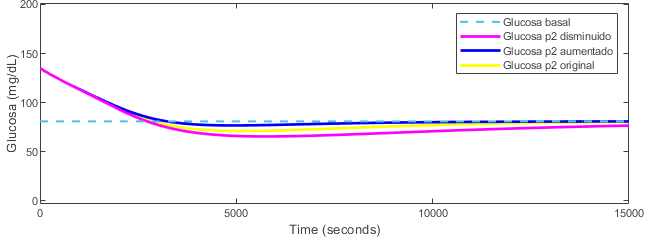
\includegraphics[width=0.9\linewidth]{img/modelo_original/p2_gl.png}
    \caption{Efecto en la glucosa de la variación de p2.}
    \label{fig:p2_gluc}
\end{figure}
\begin{figure}[htbp]
    \centering
    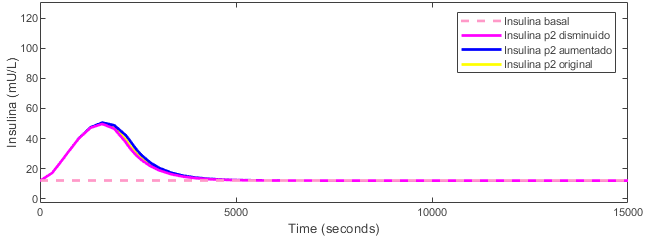
\includegraphics[width=0.9\linewidth]{img/modelo_original/p2_ins.png}
    \caption{Efecto en la insulina de la variación de p2.}
    \label{fig:p2_ins}
\end{figure}
\clearpage
Por último, se muestran en las Figuras \ref{fig:p3_gluc} y \ref{fig:p3_ins} las simulaciones correspondientes a la variación del parámetro p3 en el Modelo de Bergman.

\begin{figure}[htbp]
    \centering
    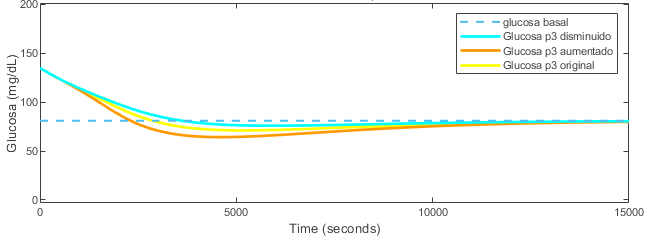
\includegraphics[width=0.9\linewidth]{img/modelo_original/p3_gl.png}
    \caption{Efecto en la glucosa de la variación de p3.}
    \label{fig:p3_gluc}
\end{figure}
\begin{figure}[htbp]
    \centering
    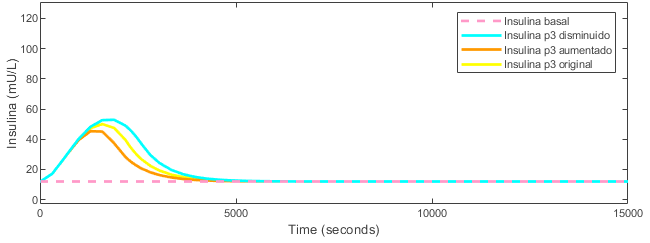
\includegraphics[width=0.9\linewidth]{img/modelo_original/p3_ins.png}
    \caption{Efecto en la insulina de la variación de p3.}
    \label{fig:p3_ins}
\end{figure}

La variación de estos dos parámetros no ha causado diferencias significativas en la glucosa y la insulina del paciente.
%\include{./tex/E_diseno}
%\apendice{Especificación de Requisitos}

Si procede.


\section{Diagrama de casos de uso}

\section{Explicación casos de uso.}

Se puede describir mediante el uso de tablas o mediante lenguaje natural.    

Una muestra de cómo podría ser una tabla de casos de uso:

% Caso de Uso 1 -> Consultar Experimentos.
\begin{table}[p]
	\centering
	\begin{tabularx}{\linewidth}{ p{0.21\columnwidth} p{0.71\columnwidth} }
		\toprule
		\textbf{CU-1}    & \textbf{Ejemplo de caso de uso}\\
		\toprule
		\textbf{Versión}              & 1.0    \\
		\textbf{Autor}                & Alumno \\
		\textbf{Requisitos asociados} & RF-xx, RF-xx \\
		\textbf{Descripción}          & La descripción del CU \\
		\textbf{Precondición}         & Precondiciones (podría haber más de una) \\
		\textbf{Acciones}             &
		\begin{enumerate}
			\def\labelenumi{\arabic{enumi}.}
			\tightlist
			\item Pasos del CU
			\item Pasos del CU (añadir tantos como sean necesarios)
		\end{enumerate}\\
		\textbf{Postcondición}        & Postcondiciones (podría haber más de una) \\
		\textbf{Excepciones}          & Excepciones \\
		\textbf{Importancia}          & Alta o Media o Baja... \\
		\bottomrule
	\end{tabularx}
	\caption{CU-1 Nombre del caso de uso.}
\end{table}

\section{Prototipos de interfaz o interacción con el proyecto.}


%\apendice{Estudio experimental}



\section{Cuaderno de trabajo.}

Enumeración de todos los métodos probados con resultados positivos o no.
\section{Configuración y parametrización de las técnicas.}

\section{Detalle de resultados.}
\apendice{Anexo de sostenibilización curricular}

\section{Introducción}

Naciones Unidas define el Desarrollo Sostenible en \cite{ONU-ODS} con el objetivo de erradicar la pobreza, proteger el planeta y asegurar la prosperidad para todos en un plazo de 15 años. Este plan se compone de 17 objetivos llamados ODS visibles en \ref{fig:sost_1}, y está incluido en la Agenda 2030, entrando en vigor el 1 de enero de 2016. Se han estudiado las asociaciones de este estudio con los OMS, estimando una especial asociación con tres de ellos, a partir de los que se muestran las siguientes consideraciones.

En primer lugar, y de forma más significativa, este estudio fomenta la salud y el bienestar del desarrollo sostenible. La comprensión, así como el avance en el conocimiento de la interacción entre la glucosa y la insulina contribuye a la mejora de la comprensión de estos sistemas, lo que a su vez conlleva al desarrollo de nuevos avances, tanto en el ámbito preventivo, como en el tratamiento, así como en la tecnología. Especial relevancia tiene, para este objetivo, la aparición de nuevos mecanismos de control de la diabetes, que pueden mejorar considerablemente el pronóstico y nivel de vida de todas las personas afectadas. Concretamente, la investigación en este campo es clave para varios aspectos. En primer lugar, la diabetes es una enfermedad crónica que puede causar numerosas complicaciones si no se trata de manera adecuada (enfermedades cardiovasculares, cardiopatía o nefropatía, entre otras). El aumento de conocimiento sobre esta patología funciona como técnica eficaz para la prevención, parte fundamental en la salud pública. Por otro lado, el desarrollo de nuevas soluciones tecnológicas, así como el descubrimiento de datos reveladores puede tener un impacto significativo en los tratamientos de la enfermedad. Esto repercute directamente en los pacientes, que podrían experimentar mejoras muy significativas en su calidad de vida, minimizando además el riesgo de complicaciones. Además, el avance médico implica la promoción de bienestar no solo para el paciente individual, sino para toda la población, independientemente de su edad, género, origen o situación socioeconómica. La expansión de estas mejoras contribuye a la universalidad del acceso a ellas. El ejercicio físico promueve la promoción de un estilo de vida activo y saludable, mostrando las mejoras que se producen al llevarlo a cabo. De esta manera, no solo se mejora la salud cardiovascular y muscular, sino que se puede reducir el riesgo de complicaciones, eje de la importancia de la salud.

Por otro lado, también se puede asociar, en menor grado, este estudio con el objetivo número 12 del Desarrollo Sostenible: Producción y Consumo responsables. Además de concienciar a la población sobre los riesgos que acarrea la enfermedad de la diabetes, aumentar la información sobre este campo permite reducir el tamaño del problema, centrando las estrategias de creación de nuevos sistemas. De esta manera se contribuye a la reducción de desperdicio de recursos médicos, así como a la optimización de su uso para tratamientos más eficientes. Este desperdicio de recursos, entre los que podrían destacar la fabricación de medicamentos y los dispositivos médicos, puede tener un impacto significativo en el medio ambiente, por lo que su reducción contribuye directamente con el consumo responsable. 

Por último, el objetivo número 9, de Industria, innovación e Infraestructura, se relaciona directamente con el desarrollo de nuevos avances, especialmente tecnológicos, de mecanismos de monitorización y control de los sistemas glucorregulatorios, como son el caso de las bombas de insulina y del páncreas artificial. Estos avances representan una forma de innovación en el campo de la medicina, así como en la gestión de enfermedades crónicas, contribuyendo al avance de la ciencia. La infraestructura, pasa primero por el aprendizaje profundo de la interacción entre la glucosa y la insulina, así como por el descubrimiento de nuevas posibles relaciones que contribuyan a la mejora de la enfermedad, especialmente en cuanto a tratamiento de la patología. La creación de estos sistemas tecnológicos contribuye, por su parte, a la creación de nuevas empresas y fomento de la industria. El fortalecimiento de la infraestructura también repercute en la atención médica, pues el desarrollo de nuevas técnicas puede reducir la duración de tratamientos, así como la duración de consultas y estudios del paciente. Al aplicar este hecho al conjunto de la sociedad, se mejora el acceso a servicios de salud de calidad, y disminuyen los conflictos médicos respecto a pocos recursos y diagnósticos.

\begin{figure}[htbp]
    \centering
    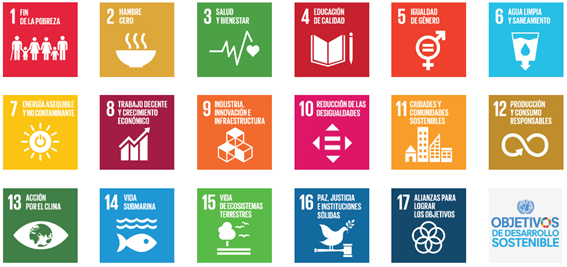
\includegraphics[width=0.9\linewidth]{img/anexos/sostenibilidad/sostenibilidad.png}
    \caption{Objetivos ODS del Desarrollo Sostenible. }
    \label{fig:sost_1}
\end{figure}



\bibliographystyle{apalike}
\bibliography{bibliografiaAnexos}

\end{document}